\chapter{Introduction and Literature Review}
\label{ch:intro_lit}

\section{Background and Motivation}
Over the past two decades, computer networking has experienced a paradigm shift driven by cloud computing, high-frequency distributed applications, and multi-tenant datacenters. In these modern environments, network traffic patterns are notoriously dynamic, characterized by extreme burstiness, unpredictable traffic matrices, and the co-existence of short, latency-sensitive RPC flows (``mice flows'') with massive, bandwidth-saturating bulk transfers (``elephant flows'').

Traditional packet forwarding protocols rely on decentralized, distributed control planes such as Open Shortest Path First (OSPF), Intermediate System to Intermediate System (IS-IS), and Border Gateway Protocol (BGP). While these protocols provide survivability across autonomous domains, they operate primarily on static link weights or slowly converging distributed metrics. Under bursty traffic conditions, static shortest-path forwarding inevitably results in localized link bottlenecks, buffer exhaustion in switch queues (bufferbloat), and severe tail-drop packet loss. When packet loss occurs, end-to-end transport protocols such as TCP Reno and TCP Cubic cut their congestion windows ($cwnd$) by half or more, triggering throughput collapse and severely degrading application service level agreements (SLAs).

Software-Defined Networking (SDN) breaks the conventional vertical integration of networking equipment by decoupling the \textit{control plane} (which decides how traffic should be handled) from the \textit{data plane} (the underlying hardware or software switches that forward packets) \cite{mckeown2008openflow, kreutz2015software}. Through standardized southbound protocols such as OpenFlow 1.3 \cite{openflow13spec}, a logically centralized controller gains global visibility over network topology, link configurations, and real-time port statistics. This centralized perspective makes it feasible to observe network state in real time and compute globally optimal forwarding decisions.

\section{Problem Formulation: The Reactive Control Lag}
Despite the promise of centralized SDN traffic engineering, existing industrial and academic approaches suffer from a fatal flaw: \textbf{they are fundamentally reactive}.

A standard reactive SDN traffic management loop functions as follows:
\begin{enumerate}[noitemsep]
  \item Switches collect byte and packet counters on their physical egress queues.
  \item The SDN controller periodically queries switches via OpenFlow multipart port-statistics request messages (\texttt{OFPMP\_PORT\_STATS}).
  \item The controller calculates instantaneous link utilization:
  \begin{equation}
    U(t) = \frac{\Delta \text{Bytes} \times 8}{C \cdot \Delta t}
  \end{equation}
  where $C$ is the physical link capacity in bits per second, and $\Delta t$ is the polling interval (typically $1.0\text{--}2.0$ seconds to prevent control-plane overload).
  \item If $U(t)$ exceeds an alarm threshold (e.g., $U(t) \ge 0.80$), the controller triggers a rerouting algorithm (e.g., Dijkstra or constrained shortest path) to move selected flows to an alternate path.
  \item The controller dispatches OpenFlow flow modification (\texttt{OFPFC\_MODIFY} or \texttt{OFPFC\_ADD}) messages to the affected switches.
\end{enumerate}

\begin{hazardbox}[The Reactive Control Lag Problem]
In high-speed networks, queue buffers are small (typically 50--200 packets in commodity switches or Mininet TCLinks to minimize latency). When an elephant flow arrives or a microburst ramps up at 10\,Gbps, the egress buffer fills in \textbf{sub-millisecond intervals}. A controller operating on a 2.0-second polling cycle observes the congestion \textbf{long after} packets have already been dropped, TCP windows have collapsed, and user latency has spiked. Reaction is not avoidance; by the time a reactive controller intervenes, the damage has already occurred.
\end{hazardbox}

\begin{figure}[H]
  \centering
  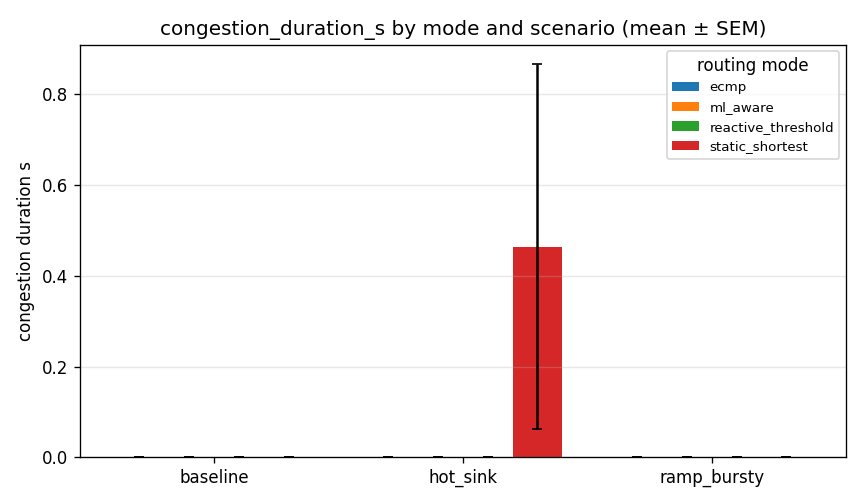
\includegraphics[width=0.54\textwidth]{results/figures/congestion_duration_s_by_scenario.png}
  \caption{Empirical link congestion duration across 46 Mininet runs. Static shortest routing experiences persistent queue saturation ($0.46\,\text{s}$ average under hot-sink, with an observed $1.854\,\text{s}$ episode), while proactive ML-Aware control completely preempts link overload, achieving $0.00\,\text{s}$ of active saturation. Under reactive rerouting, brief micro-bursts below the 2-second polling threshold registered $0.00\,\text{s}$ due to the discrete telemetry sampling quantum.}
  \label{fig:congestion_duration_intro}
\end{figure}

\section{The Core Thesis: Proactive Lead Time vs. Mere Accuracy}
A primary intellectual contribution of this project is establishing that \textbf{predictive lead time}, rather than raw classification accuracy, is the sole operational metric that matters in autonomous network traffic engineering.

In academic machine learning literature, models are frequently evaluated on global accuracy or ROC-AUC without regard to timing. However, an ML model that reports 99.9\% accuracy but forecasts a link failure only 5 milliseconds before packet drop is operationally useless to an SDN controller that requires 18 milliseconds to compute and install OpenFlow flow-mods. Conversely, a model that reliably alerts the controller \textbf{2 to 10 seconds ahead} provides sufficient timing slack to install alternate paths in a \textit{Make-Before-Break} manner, shifting flows transparently before the bottleneck queue ever bloats.

\begin{formulabox}[Operational Timing Slack Formulation]
Let $T_{\text{breach}}$ be the timestamp when link utilization physically exceeds the critical threshold $U_{\text{crit}} = 0.80$. Let $T_{\text{detect}}$ be the timestamp at which the controller ingests switch counters. In a polling-based SDN architecture with interval $T_{\text{poll}}$, the traffic surge may occur at any point within the cycle, introducing a \textbf{polling phase latency} $T_{\text{poll\_delay}} \in [0, T_{\text{poll}}]$. Let $T_{\text{infer}}$ be the machine learning inference latency ($\approx 1.2\,\text{ms}$), let $T_{\text{compute}}$ be the Dijkstra path-computation time ($\approx 0.5\,\text{ms}$), and let $T_{\text{flowmod}}$ be the OpenFlow barrier-synchronized rule installation latency across all transit switches ($\approx 18.1\,\text{ms}$).

The true \textbf{operational timing slack} $T_{\text{slack}}$ is formulated as:
\begin{equation}
  T_{\text{slack}} = (T_{\text{breach}} - T_{\text{detect}}) - (T_{\text{poll\_delay}} + T_{\text{infer}} + T_{\text{compute}} + T_{\text{flowmod}})
\end{equation}
Autonomous closed-loop congestion avoidance is physically guaranteed \textbf{if and only if}:
\begin{equation}
  T_{\text{slack}} > 0 \iff (T_{\text{breach}} - T_{\text{detect}}) > T_{\text{poll\_delay}} + T_{\text{ctrl}}
\end{equation}
where $T_{\text{ctrl}} = T_{\text{infer}} + T_{\text{compute}} + T_{\text{flowmod}} \approx 19.8\,\text{ms}$. When polling phase alignment is favorable ($T_{\text{poll\_delay}} \approx 0$), the empirical 2.005-second lead time provides generous margin ($T_{\text{slack}} \approx 1.985\,\text{s}$). However, under worst-case phase alignment ($T_{\text{poll\_delay}} \approx T_{\text{poll}} = 2.0\,\text{s}$), $T_{\text{slack}} \approx -0.015\,\text{s} \le 0$, proving that polling frequency directly bounds proactive control feasibility.
\end{formulabox}

\section{Review of Congestion Management Literature}

\subsection{End-to-End Transport Protocols and AQM}
Traditional TCP mechanisms (TCP Reno, Cubic, DCTCP \cite{alizadeh2010data}, BBR \cite{cardwell2017bbr}) operate strictly at the transport endpoints. Loss-based algorithms intentionally fill bottleneck switch buffers until tail-drop occurs, creating latency spikes and bufferbloat. Active Queue Management (RED \cite{floyd1993random}, CoDel \cite{nichols2012controlling}) marks or drops packets probabilistically to force senders to back off. However, AQM cannot shift traffic onto underutilized alternate links in rich multipath fabrics.

\subsection{Equal-Cost Multi-Path (ECMP) Limitations}
Equal-Cost Multi-Path (ECMP) \cite{hopps2000analysis} hashes packet headers (5-tuple) across $k$ equal-cost next hops:
\begin{equation}
  \text{NextHop} = \text{Hash}(\text{IP}_{\text{src}}, \text{IP}_{\text{dst}}, \text{Proto}, \text{Port}_{\text{src}}, \text{Port}_{\text{dst}}) \pmod k
\end{equation}
While ubiquitous in cloud datacenters, ECMP is load-blind. When multiple elephant flows hash to the same link, hash collisions create severe congestion while adjacent equal-cost links sit idle. Furthermore, ECMP cannot exploit non-equal-cost detours that differ in hop count by even a single metric unit.

\subsection{Machine Learning and Data Leakage Pitfalls}
Prior surveys \cite{benson2010network, curtis2011mahout} demonstrate that machine learning models in networking frequently suffer from \textbf{temporal sliding-window leakage}. When rolling features computed over overlapping windows are partitioned using naive random splits, adjacent samples share identical historical measurements. Models memorize these overlapping windows and achieve near-perfect cross-validation scores ($>99\%$), but fail completely when deployed in live networks. Our work eliminates this methodological defect via \textit{run-grouped hold-out validation}.

\subsection{Agentic AI and LangGraph in NetOps}
Recent advances in Large Language Models (LLMs) and agent frameworks \cite{langgraph2024} enable natural-language network observability. LangGraph structures autonomous reasoning into directed cyclic state graphs. Rather than issuing unverified commands, a graph-based state machine enforces strict execution boundaries, ensuring that every operational action is verified by deterministic telemetry checks before concluding.

\section{Research Objectives and Scope}
This report documents the design, implementation, and empirical validation of an autonomous SDN traffic optimization system across five core objectives:
\begin{enumerate}[label=\textbf{RO\arabic*.},noitemsep,topsep=2pt]
  \item \textbf{High-Fidelity Telemetry}: Build an OpenFlow 1.3 polling harness sampling kernel datapaths at $0.5\,\text{Hz}$ ($T_{\text{poll}} = 2.0\,\text{s}$) paired with a 2\,Hz Northbound WebSocket stream, collecting over 12,000 real labeled records without measurement duplicates or deadlocks.
  \item \textbf{Anticipatory Predictive Modeling}: Train Random Forest models under run-grouped hold-out splits, achieving verified early warning lead times exceeding 2.0 seconds.
  \item \textbf{Deterministic Make-Before-Break Detours}: Design a hazard-mitigated OpenFlow rerouting mechanism pre-programming downstream rules before shifting ingress traffic.
  \item \textbf{Agentic AI Remediation Layer}: Deploy a LangGraph StateGraph engine combining natural-language interaction, LLM risk assessment, and closed-loop verification.
  \item \textbf{Empirical Scientific Benchmarking}: Execute 46 complete Mininet \cite{lantz2010network} experiment runs on the Double Diamond topology across 3 traffic scenarios, and demonstrate wide-area multi-hop scalability on the 9-city Internet2 Abilene backbone \cite{tipper2009internet2}.
\end{enumerate}
